\documentclass[10pt]{article}
\usepackage{graphicx, fancyhdr, enumerate}
\usepackage{amsmath, amsfonts, color, multicol, mathtools}
\usepackage{blkarray}

\setlength{\topmargin}{-.55 in} 
\setlength{\textheight}{9 in}
\setlength{\textwidth}{6.625 in} 
\setlength{\evensidemargin}{-.0625 in}
\setlength{\oddsidemargin}{-.0625 in} 
\setlength{\parindent}{0 in}
\setlength{\headheight}{18.0pt}
\newcommand{\ds}{\displaystyle}
\newcommand{\xbar}{\overline{X}}

\DeclarePairedDelimiter{\ceil}{\lceil}{\rceil}

\cfoot{\thepage} 
\renewcommand{\headrulewidth}{0.4pt} 
\renewcommand{\footrulewidth}{0pt} 
\newcommand{\ansfont}[1]{{\textcolor{blue}{\textbf{Answer:}}\ \ #1}}


\lhead{\Large\sffamily Stat 330 (Fall 2016): Homework 4} 
\rhead{\sffamily Due: September 21, 2016}

% Uncomment the following line to remove answers, and comment line out to show answers:
\renewcommand{\ansfont}[1]{}


\begin{document}
\pagestyle{fancy} 
Show all of your work, and \emph{please} staple your assignment if you use more than one sheet. Write your name, the course number and the section on every sheet. 

\begin{enumerate} 
 
 
\item Consider the following function also shown in the picture.
\[ f_X(x) = \left\{ \begin{array}{cc} 
0 & |x| \ge 1 \\
-x & -1 < x \le 0 \\
x & 0< x < 1
\end{array} \right. \]

\begin{center}
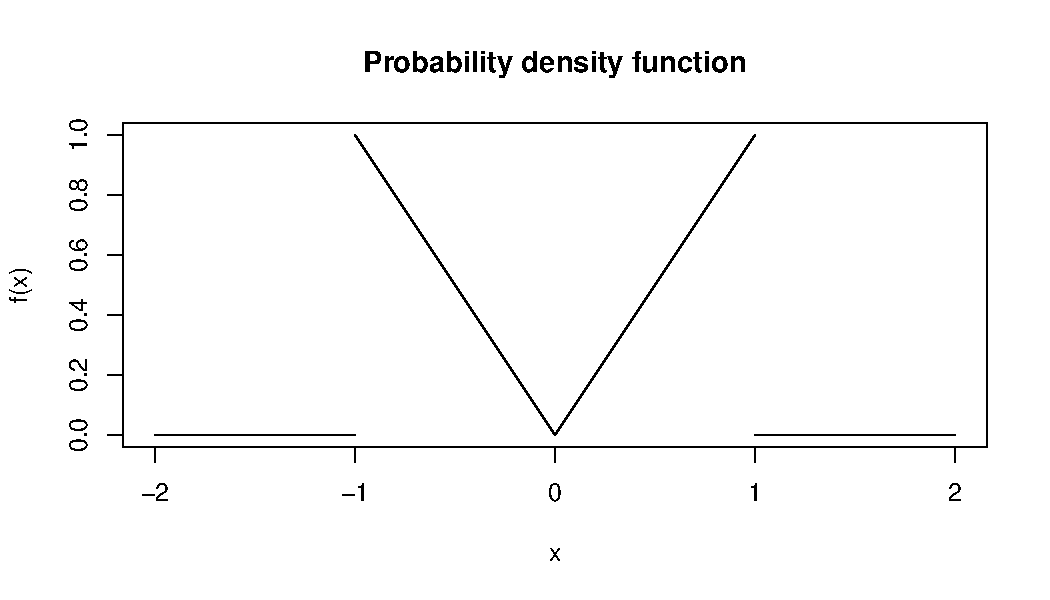
\includegraphics[scale=0.5]{plot}
\end{center}

\begin{enumerate}
\item Verify this is a valid probability density function.
\item What is the image for the random variable associated with this probability density function?
\item Derive the cumulative distribution function.
\item Calculate the expectation and variance for the random variable associated with this probability density function.
\end{enumerate}

\ansfont{
\begin{enumerate}
\item The pdf is always non-negative since it is always between 0 and 1. The integral is 
\begin{align*} 
\int_{-\infty}^\infty f_X(x) \, dx &= \int_{-1}^0 -x \, dx + \int_0^1 x \, dx  \\
&= \left. -\frac{x^2}{2}\right|_{-1}^0 +  \left. \frac{x^2}{2}\right|_0^1 \\
&= -\frac{0^2}{2} - \left(-\frac{(-1)^2}{2}\right) + \frac{1^2}{2} - \frac{0^2}{2} \\
&= \frac{1}{2}+\frac{1}{2} = 1
\end{align*} 

Since the function is nonnegative and integrates to 1, it is a valid probability density function.

\item The image for this random variable is the interval (-1,1).

\item The cumulative distribution function is 
\[ F_X(t) = \int_{-\infty}^t f_X(x) \, dx \]
we know this is zero for $t\le 1$ and 1 for $t\ge 1$ since the image is (-1,1). But we must do the integral between -1 and 1. For $-1<t\le 0$, we have 
\[
F_X(t) = \int_{-1}^t -x \, dx 
=  \left. -\frac{x^2}{2}\right|_{-1}^t = -\frac{t^2}{2} - (-\frac{(-1)^2}{2}) 
= \frac{1-t^2}{2}
\]
For $0< t < 1$, we have 
\[
F_X(t) = \int_{-1}^0 -x \, dx + \int_0^t x \, dx 
= F_X(0) + \int_0^t x \, dx   
=  \frac{1}{2} + \left. \frac{x^2}{2} \right|_0^t 
= \frac{1}{2} + \frac{t^2}{2}
\]

So, the cumulative distribution function is 
\[ F_X(t) = \left\{ 
\begin{array}{ll}
0 & t\le 1 \\
 \frac{1-t^2}{2} & -1<t\le 0 \\
 \frac{1}{2} + \frac{t^2}{2} & 0<t <1 \\
 1 & t\ge 1
\end{array}
\right. \] 


\item The expectation is 
\begin{align*} 
\int_{-\infty}^\infty x f_X(x) \, dx &= \int_{-1}^0 x(-x) \, dx + \int_0^1 x(x) \, dx  \\
&=  \left. -\frac{x^3}{3}\right|_{-1}^0 +  \left. \frac{x^3}{3}\right|_0^1 \\
&= -\frac{0^3}{3} - \left( -\frac{(-1)^3}{3} \right) + \frac{1^3}{3} - \frac{0^3}{3} \\
&= -\frac{1}{3} + \frac{1}{3} = 0
\end{align*}
Intuitively we could have determined this expectation as the center of gravity as in Figure 3.3 in the book.

The variance is 
\begin{align*} 
\int_{-\infty}^\infty (x-E[X])^2 f_X(x) \, dx &= \int_{-\infty}^\infty x^2 f_X(x) \, dx \\
&= \int_{-1}^0 -x^3 \, dx + \int_0^1 x^3 \, dx  \\
&=  \left. -\frac{x^4}{4}\right|_{-1}^0 +  \left. \frac{x^4}{4}\right|_0^1 \\
&= -\frac{0^4}{4} - \left( -\frac{(-1)^4}{4} \right) + \frac{1^4}{4} - \frac{0^4}{4} \\
&= \frac{1}{4} + \frac{1}{4} = \frac{1}{2}
\end{align*}
\end{enumerate}
}

 \item (Baron's book): 4.2

    \ansfont{
      \newline
      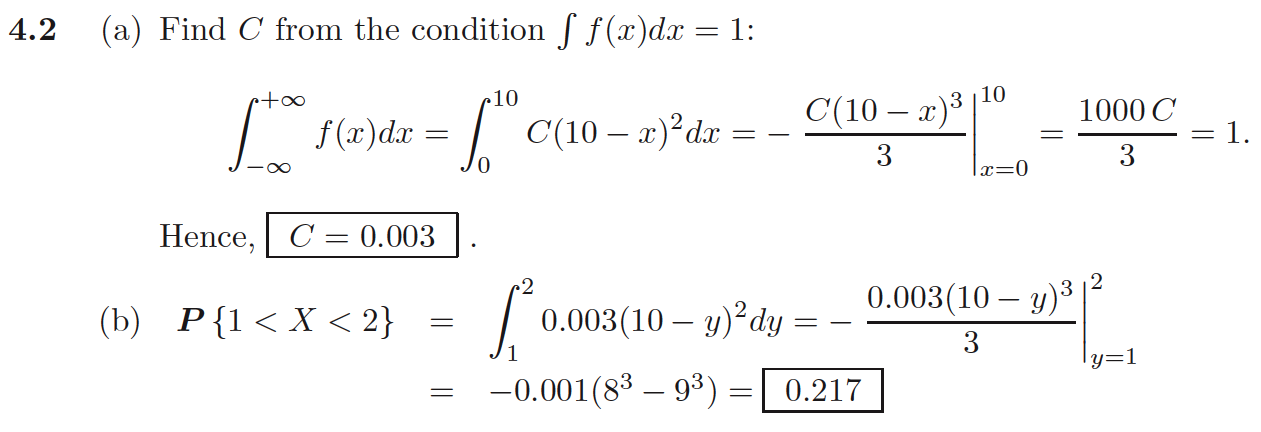
\includegraphics[width=0.8\textwidth]{baron4-2}
    }


\item A web page is accessed at an average of 10 times an hour. Assume that waiting time until the next hit has an exponential distribution and that the hits are independent of each other. 
\begin{itemize}
\item[(a.)] Determine the rate parameter $\lambda$ of the distribution of the time until the first hit?
\item[(b.)] What is the expected time between hits?
\item[(c.)] What is the distribution of the time until the second hit? (Give the name of the distribution and the value(s) of parameter(s).) 
\item[(d.)] What is the probability that the next hit is within 10 minutes?
\item[(e.)] Describe the distribution of the total waiting time for 10 hits?  (Give the name of the distribution and the value(s) of parameter(s).)
 \item[(f.)] What is the expected total waiting time for 10 hits on the web page?
\item[(g.)] What is the probability that there will be less than 10 hits in the first hour?
\end{itemize}

\ansfont{
\begin{enumerate}
\item Let $X$ be the time until the next hit. It is the same as the time between hits. By the the description, the rate parameter (number of hits per hour ) $\lambda=10$. Alternatively, the expected waiting time between hits, $E[X]= 1/10 =1/\lambda$ giving $\lambda=10$.
\item Since $X \sim Exp(10)$, we have $E[X] =1/\lambda= 1/10=.1$ (hours)
\item The time until the second hit is $Y=X_1+X_2$ where $X_1 \sim Exp(10)$ and $X_2 \sim Exp(10)$ and $X_1$ and $X_2$ are independent. Thus $Y \sim Gamma(2,10)$ (or $Erlang(2,10)$).
\item Need $P(X\le 10/60)$ where $X \sim Exp(10)$ Using the cdf  for the exponential distribution
$Exp_{10}(.16667)= 1- e^{-.16667\times 10}=1-.18888=.8111$
\item The waiting time for 10 hits is $W=\sum_{i=1}^{10}=X_i$; so $W \sim Gamma(10,10)$ (or $Erlang(10,10)$).
\item We need $E[W]$ which is given by $k/\lambda=10/10=1$ hour, as one might expect!
\item Let $N$ be the number of hits in the first hour and assume $N \sim Poi(10 \times 1)$. The we need $ P(N <10) = P(N\le 9)=0.45793$.
\end{enumerate}
}


 \item An autopilot attempts to maintain an airplane's altitude at a constant
    18000 feet. Because of random variations, the actual altitude X is a normal
    random variable with mean 18000 feet and variance=2500 $feet^2$.
    \begin{enumerate}
      \item What is the probability that the altitude differs from the assigned 18000 value by
        more than 100 feet?
      \item Suppose that by mechanically improving the autopilot,
        the variance of the airplane's altitude can actually be
        reduced. Find the value of the variance such that the probability that the altitude differs from the assigned 18000
        value by more than 100 feet is at most 0.01.
    \end{enumerate}
    \ansfont{
      \begin{enumerate}
        \item 
          Given $ X \sim N(18,000,\,2500)$, we need to calculate $P(|X-18000|>100)$:
          \begin{eqnarray*}
            P(|X-18000|>100) & = & P(X<17,900\ \text{or}\ X>18,100)\\
            & = & 1- P(17,900<X<18,100)\\
            & = & 1- P\left(\frac{17,900-18,000}{50}<Z<\frac{18,100-18,000}{50}\right)\\
            & = & 1- P(-2<Z<2)=1-(\Phi(2)-\Phi(-2))\\
            & = & 1-(0.9772-0.0228)=1-0.9544=0.0456
          \end{eqnarray*}
        \item
          Need to find $\sigma$ so that 
          \begin{align*}
            P\left( |X-18000| >100 \right) &\le 0.01\\
            P\left( |X-18000| \le 100 \right) &> 0.99\\
           P\left(\frac{17,900-18,000}{\sigma}<Z<\frac{18,100-18,000}{\sigma}\right)&> 0.99
          \end{align*}
          or, equivalently
          $$ P\left(\frac{-100}{\sigma}<Z<\frac{100}{\sigma}\right)> 0.99$$
          implying that we need $100/\sigma>2.575$, noting that
          $\Phi(2.575)-\Phi(-2.575)=0.99$. This gives $\sigma<38.835$, which
          implies $\sigma^2<1508.16$.
      \end{enumerate}
    }

\newpage
 \item Suppose that prices of a brand of television are normally distributed with mean \$400 and standard deviation \$60. 
    \begin{enumerate}
      \item What is the probability that a randomly selected television of this brand costs more than \$450?
      \item What is the probability that a randomly selected television of this brand costs between \$320 and \$420?
      \item If a particular television is cheaper than 90\% of all other televisions of this brand, how much does it cost?
      \item Suppose that prices for a different brand of television are normally distributed with mean \$300 and standard deviation \$40. If one television of each brand is purchased independently, what is the probability that the sum of the prices is less than \$600?
    \end{enumerate}
    \ansfont{
      \begin{enumerate}
        \item 
          Let $ X \sim N(400,\,3600)$. Then
          \begin{eqnarray*}
            P(X>450) & = &1- P(X<450)\\
            & = & 1- P\left(Z<\frac{450-400}{60}\right)\\
            & = & 1- P\left(Z<\frac{5}{6}\right)=1-(\Phi\left(\frac{5}{6}\right)\\
            & = & 1-(0.7977)= 0.2023.
          \end{eqnarray*}
          \item
          \begin{eqnarray*}
            P(320<X<420) & = & P\left(\frac{320-400}{60}<Z<\frac{420-400}{60}\right)\\
            & = & P\left(-\frac{4}{3}<Z<\frac{1}{3}\right)=\Phi\left(\frac{1}{3}\right)-\Phi\left(\frac{-4}{3}\right)\\
            & = & 0.630559-0.0912113=0.5393
          \end{eqnarray*}       
        \item
          We need to find $X$ such that $P(X<X*)=0.1$ For a standard normal random variable, $Z$, we have $P(Z<Z*)=0.1$ for $Z*=-1.28155$. So $X*=60Z*+400=60(-1.28155)+400=\$323.11$.
      \item Let $S$ denote the price of the two different televisions. Since the purchases are independent, $S\sim N(400+300, 60^2+40^2)$. Then, 
      \begin{eqnarray*}
            P(S<600) & = & P\left(Z<\frac{600-700}{\sqrt{5200}}\right)\\
            & = &  \Phi\left(\frac{600-700}{\sqrt{5200}}\right) \\
            & = & 0.0828
          \end{eqnarray*}
                \end{enumerate}
    }



\item (Baron's book): 4.19

    \ansfont{
      \newline
      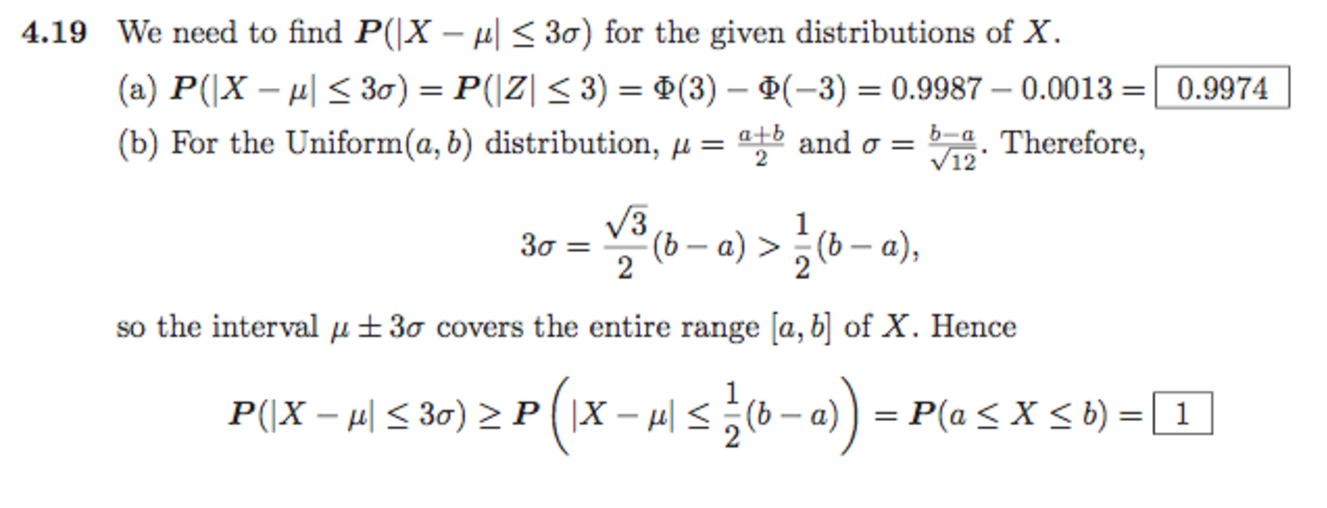
\includegraphics[width=0.8\textwidth]{baron4-19}
    }
          
  
\end{enumerate}
\end{document}
